\section{Schwellwertschemata}

\label{sec_basics_threshold}

%- Shamir How to share a secret?
%- Public Key Problematik
%- Was ist das? (siehe auch Paper für Definition)
%- Fünde (RSA, Paillier, ...) und Desmedt/Frankel evtl. hier schon Pedersen/...

Mit der Verbreitung technischer Systeme, die kryptographische Verfahren nutzen, in den 70er Jahren musste auch das Problem der sicheren Aufbewahrung und Verteilung kryptographischer Schlüssel betrachtet werden. Die Sicherheit dieser Schlüssel ist essentiell für den Betrieb solcher Systemen. Das einfache Speichern eines Schlüssels an einem einzigen Ort resultiert in einer hohen Verlustwahrscheinlichkeit, da ein einzelner Fehler wie unbeabsichtigtes Löschen oder Speichermedienausfall den Schlüssel unwiederbringlich verloren gehen lassen kann. Das mehrfache Speichern eines Schlüssels an verschiedenen Orten erhöht hingegen die Gefahr eines Schlüsseldiebstahls oder -missbrauchs, da auch die Angriffsoberfläche vergrößert wird. Bei möglichen Lösungen dieses Problems müssen also immer die Integrität und die Vertraulichkeit eines Schlüssels gegeneinander abgewogen werden. \cite{gemmell1997}

Ausgehend von diesen Überlegungen entwickelte Shamir das erste \((k,n)\)-Schwellwertschema: Ein Geheimnis \(D\) wird so in \(n\) Teile \(D_1, \dots, D_n\) (\textit{Shares}) zerlegt, dass durch Kenntnis von mindestens \(k\) Teilen das Geheimnis wieder aufgedeckt werden kann, aber jede Kombination aus höchstens \(k-1\) Teilen keine Informationen über \(D\) liefert \cite{shamir1979}.\footnote{
  Im selben Jahr veröffentlichte auch Blakley eine Lösung dieses Problems, die auf den Schnittpunkten von Hyperebenen über endlichen Feldern beruht \cite{blakley1979}.
} 

Auf Basis dieses Verfahrens kann also die Integrität eines Schlüssels erhöht werden, da nun selbst bei Verlust von \(n-k\) Teilen der Schlüssel noch wiederhergestellt werden kann. Auf der anderen Seite ist die Vertraulichkeit jedoch höher als bei der mehrfachen Speicherung des Schlüssels im Original, da mindestens \(k\) Teile des Schlüssels zur Wiederherstellung vorliegen müssen.

Shamirs Verfahren wird im Folgenden im Detail beschrieben, da es auch im später erläuterten und verwendeten Schwellwertschema eine wichtige Rolle spielt.

\subsection*{Shamir's Secret Sharing}

Die Menge aller Ganzzahlen modulo einer Primzahl \(p\) bilden den (endlichen) Körper \(\mathbb{Z}_p\), dessen Eigenschaften für das Verfahren entscheidend sind. Soll das Geheimnis \(D\) (das o.B.d.A. als Ganzzahl angenommen wird) aufgeteilt werden, so wird eine Primzahl \(p\) mit \(p > D\) und \(p > n\) gewählt. Weiterhin wird ein Polynom 
\[q(x) = a_0 + a_1x + \dots + a_{k-1}x^{k-1} \text{ mit } a_0 = D\] 
derart gewählt, dass \(a_1, \dots, a_{k-1}\) zufällig gleichverteilt aus der Menge \(\mathbb{Z}_p \setminus \{0\}\) stammen. Die einzelnen \textit{Shares} werden nun als
\[D_1=(x_1,q(x_1)), \dots, D_i=(x_i,q(x_i)), \dots, D_n=(x_n,q(x_n))\]
jeweils modulo \(p\) berechnet, wobei die \(x_i\) paarweise unterschiedlich aus \(\mathbb{Z}_p\) gewählt werden können. Beispielsweise kann schlicht \(x_i = i\) gelten.\todo{Vielleicht diese Werte direkt nutzen?}

Um nun aus diesen einzelnen Teilen wieder das ursprüngliche Geheimnis zu erhalten, wird das Verfahren der Langrange'schen Polynominterpolation verwendet, das ausgehend von einer Menge von Punkten ein Polynom findet, das durch diese Punke verläuft. Hierbei wird die Tatsache ausgenutzt, dass jedes Polynom vom maximalen Grad \(t-1\) in einem mathematischen Körper durch \(t\) Punkte exakt bestimmt wird.

Für die zur Rekonstruktion verwendeten \(t\) Teile \(D_1'=(x_1',q(x_1')),\dots,D_t'=(x_t',q(x_t'))\) werden \(t\) Werte \todo{mod p irgendwo erwähnen}
\[\lambda_i := \prod_{j=1, j \not= i}^{t} \; \frac{- x_j'}{x_i' - x_j'} \text{ für } i \in \{1,\dots,t\}\] 
definiert. Das gesuchte Geheimnis \(D\) kann nun als
\[D = \sum_{i=1}^{t}\lambda_i \cdot q(x_i')\]
berechnet werden. Da \(\lambda_i\) nicht von \(q(x_i)\) abhängt, können diese Werte in der Praxis bereits vorberechnet werden. Details zu der Korrektheit dieses Verfahrens sind \cite{boneh2016} zu entnehmen.

Das Problem dieser Lösung bezogen auf den in dieser Arbeit behandelten Anwendungsfall ist jedoch, dass das Geheimnis nach erstmaligem Aufdecken bekannt ist. Wünschenswert wäre ein Verfahren, bei dem nur ein entsprechend verschlüsseltes Datum (bspw. der gesuchte Eintrag in einer Pseudonym-Tabelle) aufgedeckt werden kann, ohne dass der kombinierte Schlüssel selbst bekannt wird. 

\subsection*{Threshold Decryption}

%- 87 SocietyOriented \cite{desmedt1987}
%- 93 Threshold decryption (non-interactive) \cite{desmedt1993}
%- Def. nach 96 Boneh \cite{boneh2006}

In \cite{desmedt1987} wird das erwähnte Problem das erste Mal im Kontext von verschlüsselten Nachrichten an Gruppen betrachtet: Ein Sender möchte eine Nachricht an eine Gruppe von Empfängern senden, die nur in Zusammenarbeit die Nachricht entschlüsseln können sollen. Hier wird auch die zentrale Forderung an mögliche Lösungen des Problems aufgestellt, den mehrfachen Nachrichtenaustausch zwischen Sender und Empfänger(n) bei der Entschlüsselung (sogenannte Ping-Pong-Protokolle) zu vermeiden. 

In \cite{desmedt1993} spricht der Autor bei dieser Klasse von Verfahren von \textit{Threshold Decryption} und fordert weiterhin, dass praktisch einsatzbare Systeme auch \textit{non-interactive} sein sollten, also bei der Entschlüsselung keinen aufwendigen Datenaustausch zwischen den Besitzern der \textit{Shares} notwendig machen.

\begin{figure}[]
    \centering
        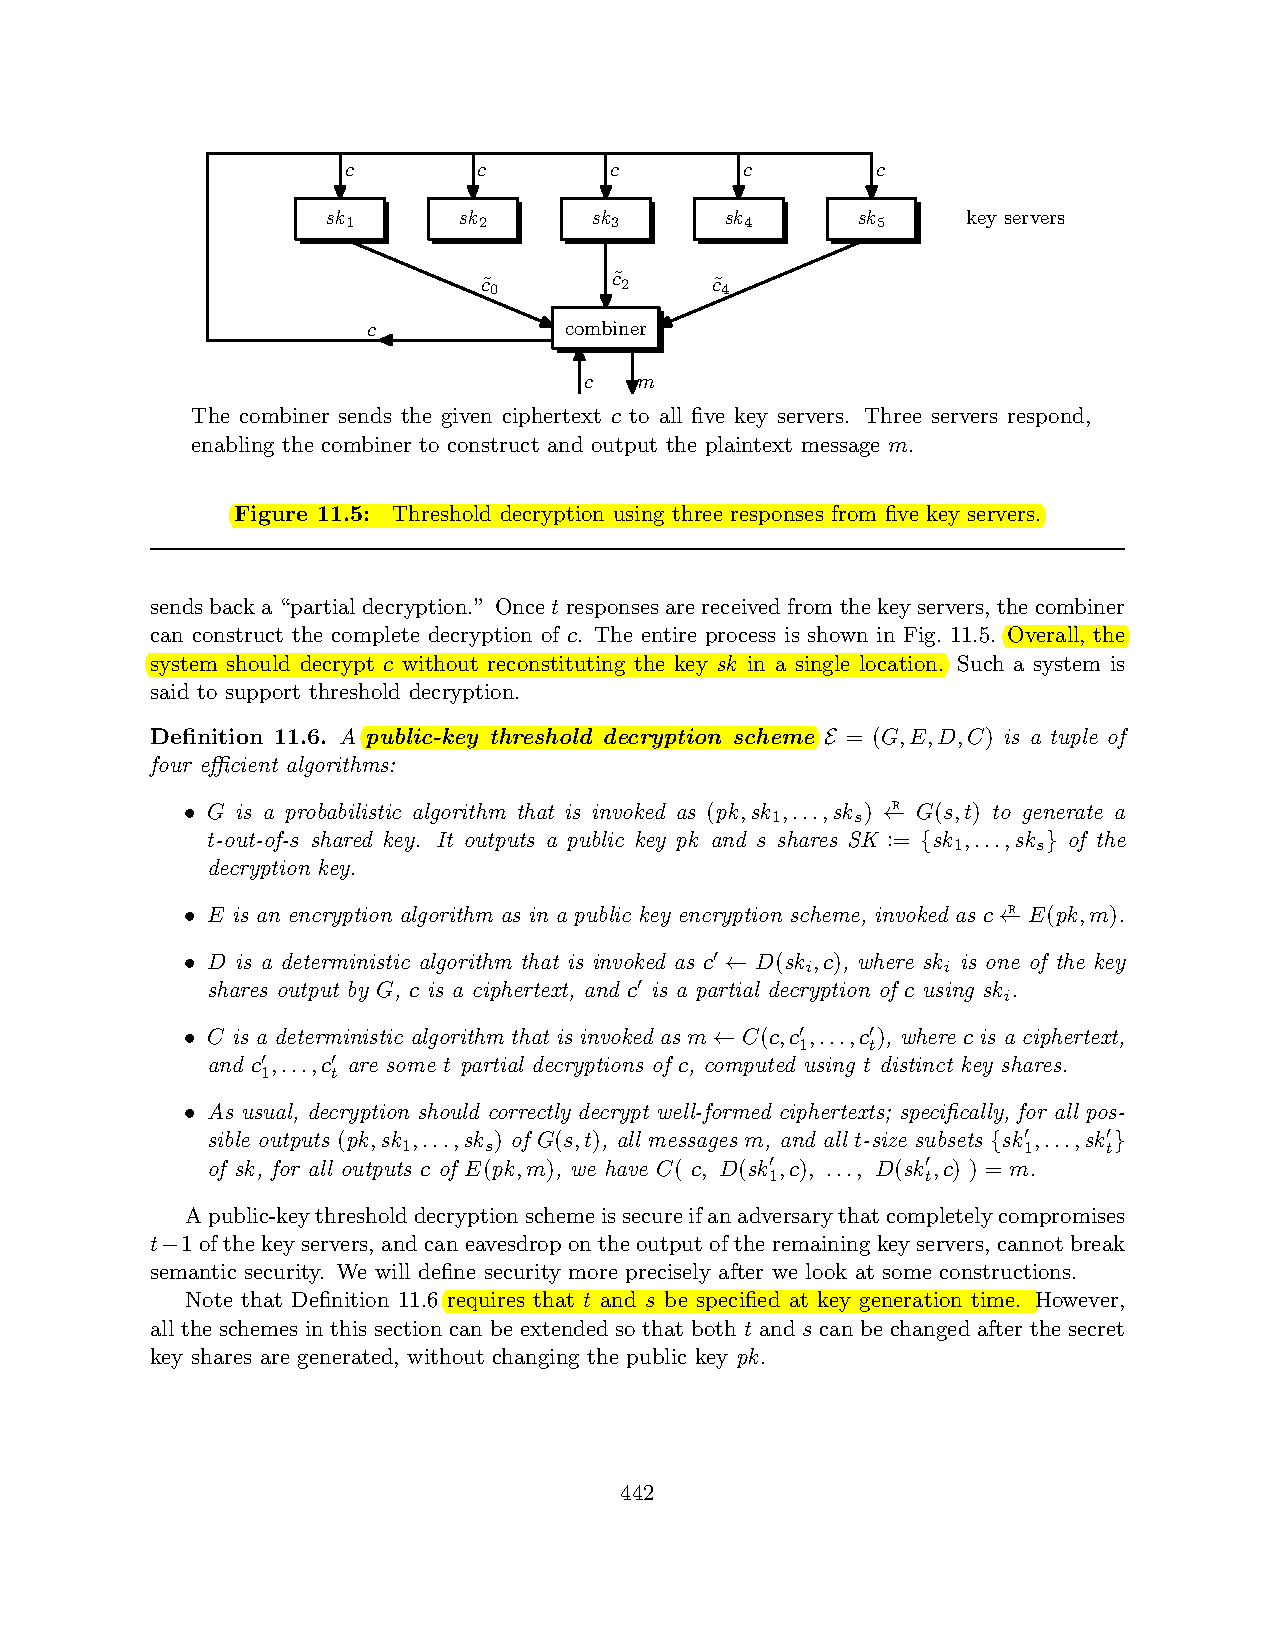
\includegraphics[clip, trim=3cm 21.2cm 3cm 2cm, width=1.00\textwidth]{img/threshold_decryption_excerpt.pdf}
    \caption{Übersicht über den Entschlüsselungsvorgang bei der Nutzung eines (3,5)-Schwellwertschemas. Entnommen aus \cite{boneh2016}.}
    \label{fig:threshold_decryption_combiner}
\end{figure}

In \cite{boneh2016} werden diese Systeme formalisiert. Ein \textit{Threshold-Public-Key-Decryption}-Schema \(\epsilon = (G, E, D, C)\) besteht aus vier Algorithmen: 

\begin{itemize}
  \item \(G(t, n, r)\) ist der Algorithmus zur Generation des öffentlichen Schlüssels \(pk\) und der \(n\) \textit{Shares} des geheimen Schlüssels \(\{sk_1, \dots, sk_n\}\). \(t\) steht für die Anzahl der zur Entschlüsselung benötigten \textit{Shares}, wie bereits beschrieben. \(r\) ist als stellvertretend für die einfließenden Zufallswerte zu betrachten.
  
  \item \(E(pk, m, r)\) steht für den Algorithmus, der der Verschlüsselung einer Nachricht \(m\) mit dem öffentlichen Schlüssel \(pk\) dient. \(r\) dient der Vermeidung von \textit{Known-Ciphertext-Angriffen}. \todo{Vmtl.? Mehr Details...}
  
  \item \(D(sk_i, c)\) ist der Algorithmus der für einen bestimmten \textit{Share} und einen Schlüsseltext \(c\) eine partielle Entschlüsselung \(c_j'\) liefert.
  
  \item \(C(c, c_1', \dots, c_t')\) ist der Algorithmus, der aus dem Schlüsseltext \(c\) und aus \(t\) durch \(D\) generierten partiellen Verschlüsselungen wieder die Nachricht \(m\) liefert. Dieser Algorithmus wird auch \textit{Combiner} genannt. 
\end{itemize}

Zusätzlich wird von diesen Algorithmen die folgende Eigenschaft verlangt. Sie beschreibt die korrekte Entschlüsselung von validen Schlüsseltexten im Kontext eines Schwellwertschemas: Für alle möglichen Ergebnisse \((pk, \{sk_1, \dots, sk_n\})\) von \(G\), alle möglichen Nachrichten \(m\) und alle \(t\)-elementigen Teilmengen der \textit{Shares} \(\{sk_1', \dots, sk_t'\}\) soll für alle möglichen Schlüsseltexte \(c=E(pk, m, r)\) gelten: \(C(c, D(sk_1', c), \dots, D(sk_t', c)) = m\).

Eine Übersicht über den Entschlüsselungsvorgang ist in Abbildung \ref{fig:threshold_decryption_combiner} zu finden. Dort sind die partiellen Entschlüsselungen und der \textit{Combine}-Vorgang eines \((3,5)\)-Schwellwertschemas dargestellt. Der Algorithmus \(D\) für die partielle Entschlüsselung läuft dabei auf den einzelnen \textit{Key-Servern} ab.

In \cite{boneh2006} werden diese Algorithmen noch um einen fünften erweitert, der dazu dient, einzelne partielle Entschlüsselungen auf Validität zu überprüfen. Hierdurch können fehlerhaft handelnde \textit{Key-Server} aufgedeckt werden. Hierzu wird auch der Algorithmus \(G\) verändert, der zusätzlich einen Validierungsschlüssel \(vk\) liefert:
\begin{enumerate}
	\item \(G(t, n, r)\) liefert nun \((pk, vk, \{sk_1, \dots, sk_n\})\).
  \item[...] 
  \setcounter{enumi}{4}
	\item \(V(pk, vk, c, c_j')\) überprüft die \(j\)-te partielle Entschlüsselungen auf Validität.
\end{enumerate}

Weiterhin wird für den neuen Algorithmus eine weitere Eigenschaft verlangt. Für jeden Schlüsseltext \(c\) und \(c_j' = D(sk_i,c)\), wobei \(sk_i\) der \(i\)-te von \(G\) erstellte \textit{Share} ist, gelte: \(V(pk, vk, c, c_j')\) liefert ein valides Ergebnis.